\section{Synch, Cond Vars, Scheduling}
Two main uses of synchronization: critical section problem, order of thread exec.
By threads in the same address space, local variables are \textit{private}, but
global variables, static objects, dynamic objects, and things on the heap are
\textit{shared}.
\begin{lstlisting}[basicstyle=\tiny,language=c]
// Peterson's Algorithm
int turn, flags[2];
// flags initial: [0,0]. used to show interest

func work(id_t id) // id 0 or 1
  flag[id] = 1; // true
  turn = id;
  while (turn == id && flag[1-id]) {} 
  // critical section goes here ...
  flag[id] = 0; // exit section
  // remainder section goes here ...
\end{lstlisting}
\begin{lstlisting}[basicstyle=\tiny, language=c]
// Bakery
int choosing[NUM_THREADS], number[NUM_THREADS];
func work(id_t id)
  choosing[id] = 1; // entering a `critical section'
  number[id] = max(number) + 1;
  choosing[id] = 0; // exiting a `critical section'
  for (int j = 0; j < NUM_THREADS; j++)
  { // (a,b) < (c,d) <=> (a < c) || (a == c && b < d)
    while (choosing[j]) {}   
    while (number[j] != 0 
      && ((number[j], j) < (number[i],i))) {}
  }
  // critical section goes here
  number[id] = 0; // exit section
\end{lstlisting}

\subsection*{Semaphores}
These include an integer \textit{counter}, accessed through an atomic
{\tt wait (decrement, P)} and {\tt signal (increment, V)}, and a queue of
waiting threads. There are two types, \textit{binary/mutex} and
\textit{counting semaphore}. The binary works the same as a lock (locks have
owners, semaphores dont). The counting
semaphore is a resource with many units avaialble that allows certian kinds of
unsynchronized concurrent accesses (like reading). Multiple threads can pass
the semaphore, and the max num of threads is determined by the intitial. Atomic
instructions are done through \textbf{test-and-set}, which does
{\tt 
bool testAndSet(bool *lock): bool old = *lock; *lock = true; return old
}.

Problems with machine insructions: 1. starvation is possible, 2. deadlock is
possible through priority inversion.


\subsection*{Condition Variables}
CVs keep a queue of waiting threads, and have three atomic operations,
{\tt cvWait(cv *cv, mtx *mutex)}, releases lock, waits, and reacquires before
return), {\tt cvSignal(cv *cv) }, which wakes one enqueed thread, and {\tt
cvBroadcast(cv *cv)}, which wakes all enqueued threads. CVs are \textit{always used with locks}, the locks protect the shared data being modified and tested when deciding wheter to wait or signal/broadcast
\begin{lstlisting}[basicstyle=\tiny, language=c]
lock_acquire(lock);
while (condition not true) { cv_wait(cond, lock); }
// do stuff
cv_signal(cond); // or cv_broadcast(cond);
lock_release(lock);
\end{lstlisting}
\textbf{Monitors} enforce mutual exclusion, since local data is only accessed by the monitor's procedures. A process enters the monitor by invoking one of its procedures. Other processes are blocked.
If process $P$ executes $x.signal$ operation and $\exists$ a suspended proccess
$Q$ that is associated with condition $x$, then we have an issue, so we use
\textbf{Hoare} and \textbf{Mesa} semantics to deal with this. To use monitors in 
C, you need a bounded buffer of size $N$, a function {\tt addToBuffer()} and
{\tt removeFromBuffer()}, one lock (only lock holder is allowed to be active in
one of the monitors functions), and two CVs, one to make producers wait, one to
make consumers wait.
Pattern for using monotirs
    1. acquire lock
    2. call {\tt cvWait()} only inside {\tt while()} loop (mesa)
    3. whenever a CV being waited on might have changed (F to T), signal
    corresponding CV.
    4. release the lock on the monitor.

\subsection*{Scheduling}
The goals of scheduling are fairness (each thread gets a fair-but not
necessarily equal- share of the CPU), avoid starvation, enforce the policy, and
balane (all parts of the system buys). \textbf{batch systems} maximize jobs
completed per hour, and minimize turnaround time (time between submission and
completion), and keep the cpu busy all the time. \textbf{interactive systems}
minimize time between recieving request and \textit{starting} to produce
output, and are proportional (ie simple tasks complete quickly). \textbf{real
time} systems are predictable and meet deadlines. sometimes these systems
conflict with each other. Types of CPU scheduling include \textit{admission
scheduling/control} (used in batch systems), \textit{medium-term/memory
scheduling} (decides which processes are swapped out to disk), and
\textit{short term scheduling} (dispatching), which needs to be efficient.
Dispatching is called \textbf{context switching}, where current state is
saved, and the next thread is restored. A thread is scheduled when it enters
the ready state, when the running thread blocks (or exits) or at fixed
intervals. Two types of scheduling are \textit{non-preemptive} schduling (once
CPU is allocated to a thread, it keeps the CPU until it terminates -- good for
batch), and \textit{preemptive} scheduling, where the cpu can be taken froma thread and
allocated to another
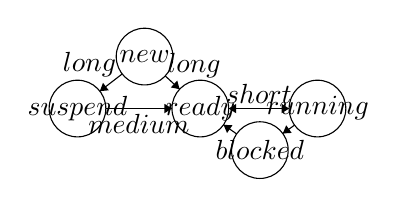
\begin{tikzpicture}[scale=0.12]
\tikzstyle{every node}+=[inner sep=0pt]
\draw [black] (15.8,-10.8) circle (3);
\draw (15.8,-10.8) node {$suspend$};
\draw [black] (22.9,-5.3) circle (3);
\draw (22.9,-5.3) node {$new$};
\draw [black] (28.8,-10.8) circle (3);
\draw (28.8,-10.8) node {$ready$};
\draw [black] (41.2,-10.8) circle (3);
\draw (41.2,-10.8) node {$running$};
\draw [black] (35.1,-15.2) circle (3);
\draw (35.1,-15.2) node {$blocked$};
\draw [black] (18.8,-10.8) -- (25.8,-10.8);
\fill [black] (25.8,-10.8) -- (25,-10.3) -- (25,-11.3);
\draw (22.3,-11.3) node [below] {$medium$};
\draw [black] (20.53,-7.14) -- (18.17,-8.96);
\fill [black] (18.17,-8.96) -- (19.11,-8.87) -- (18.5,-8.08);
\draw (17.07,-7.55) node [above] {$long$};
\draw [black] (25.09,-7.35) -- (26.61,-8.75);
\fill [black] (26.61,-8.75) -- (26.36,-7.84) -- (25.68,-8.57);
\draw (28.14,-7.57) node [above] {$long$};
\draw [black] (31.8,-10.8) -- (38.2,-10.8);
\fill [black] (38.2,-10.8) -- (37.4,-10.3) -- (37.4,-11.3);
\draw (35,-10.3) node [above] {$short$};
\draw [black] (38.2,-10.8) -- (31.8,-10.8);
\fill [black] (31.8,-10.8) -- (32.6,-11.3) -- (32.6,-10.3);
\draw [black] (38.77,-12.56) -- (37.53,-13.44);
\fill [black] (37.53,-13.44) -- (38.47,-13.38) -- (37.89,-12.57);
\draw [black] (32.64,-13.48) -- (31.26,-12.52);
\fill [black] (31.26,-12.52) -- (31.63,-13.39) -- (32.2,-12.57);
\end{tikzpicture}
\begin{itemize}
  \item FCFS. Each process runs to completion when it arrives.
  \item SJF (shortest job first). Pick the job with the shortest service time.
  \item Round Robin. There is a fixed time slice. A process gets placed at the
end of the ready queue. A process that finishes its time slice get placed in
the ready queue as well.
  \item Priority Scheduling. A priority $p$ is associated with each thread. The
thread with $max(p)$ in the ready queue is picked. This policy could suffer
from \textbf{priority inversion} or \textbf{starvation}.
  \item Multily level queue. Multiple ready queues, where a runnable thread is
    only on one queue. Threads are permanently assigned to a queue, and each
    thread has its own scheduling algorithm (usually RR), and another
    scheduling policy chooses which queue goes next (usually priority based).
  \item MLFQ. dynamically choose a thread based on past history. this boosts
    priorty of threads that have waited a long time, and can prefer threads
    that dont use their full quanta, or threads following a user input.
  \item Fair Share. Group threads by user/department. Ensure each group gets a
    proportional share of the CPU, priority of thread depends on its own
    priority and the history of the group. Lottery scheduing variant, where
    each group is assigned tickets, and lotteries are held to find next
    process.
  \item Unix Scheduling. Interactive threads favored. more cpu accumulation
    lowers priority, aging prevents starvation.
\end{itemize}


